\chapter{Week 3}
\section{Logistic Regression}
Now we are switching from regression problems to {\bf classification problems}. Don't be confused by the name ``Logistic Regression"; it is named that way for historical reasons and is actually an approach to classification problems, not regression problems.
\section{Binary Classification}
Instead of our output vector y being a continuous range of values, it will only be 0 or 1.
\[y \in \{0,1\} \]
Where 0 is usually taken as the ``negative class" and 1 as the "positive class", but you are free to assign any representation to it.

We're only doing two classes for now, called a ``Binary Classification Problem."

One method is to use linear regression and map all predictions greater than 0.5 as a 1 and all less than 0.5 as a 0. This method doesn't work well because classification is not actually a linear function.

Hypothesis Representation

Our hypothesis should satisfy:
\[0 \leq h_\theta (x) \leq 1 \]

Our new form uses the {\bf ``Sigmoid Function"}, also called the {\bf ``Logistic Function"}:
\begin{align}
h_\theta (x) &=  g ( \theta^T x ) \\
z &= \theta^T x \\
g(z) &= \dfrac{1}{1 + e^{-z}}
\end{align}

\begin{figure}[ht]
\center
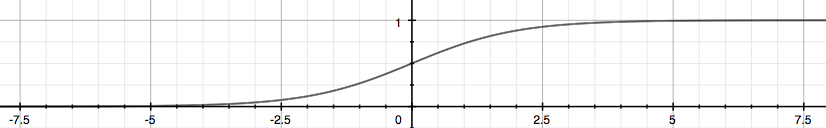
\includegraphics[scale=0.5]{W3_sigmoid}
\caption{Sigmoid Function}
\label{fig:W3_sigmoid}
\end{figure}

The function g(z), shown here, maps any real number to the (0, 1) interval, making it useful for transforming an arbitrary-valued function into a function better suited for classification. Try playing with interactive plot of sigmoid function: \href{https://www.desmos.com/calculator/bgontvxotm}{click here!}.

We start with our old hypothesis (linear regression), except that we want to restrict the range to 0 and 1. This is accomplished by plugging $\theta^T $ into the Logistic Function.

$h_\theta $ will give us the probability that our output is 1. For example, $h_\theta(x)=0.7$ gives us the probability of 70\% that our output is 1.

\begin{align*}
&h_\theta(x) = P(y=1 | x ; \theta) = 1 - P(y=0 | x ; \theta) \\ 
&P(y = 0 | x;\theta) + P(y = 1 | x ; \theta) = 1
\end{align*}

Our probability that our prediction is 0 is just the complement of our probability that it is 1 (e.g. if probability that it is 1 is 70\%, then the probability that it is 0 is 30\%).
\section{Decision Boundary}
In order to get our discrete 0 or 1 classification, we can translate the output of the hypothesis function as follows:
\begin{align*}
& h_\theta(x) \geq 0.5 \rightarrow y = 1 \\
& h_\theta(x) < 0.5 \rightarrow y = 0 \\
\end{align*}
The way our logistic function g behaves is that when its input is greater than or equal to zero, its output is greater than or equal to 0.5:
\begin{align*}
g(z) \geq 0.5 \\
\text{when } z \geq 0
\end{align*}
Remember:
\begin{align*}
z=0,  e^{0}=1 \Rightarrow  g(z)=1/2\\ 
z \to \infty, e^{-\infty} \to 0 \Rightarrow g(z)=1 \\ 
z \to -\infty, e^{\infty}\to \infty \Rightarrow g(z)=0 
\end{align*}

So if our input to g is $\theta^T$, then that means:
\begin{align*}
& h_\theta(x) = g(\theta^T x) \geq 0.5 \\
& \text{when} \; \theta^T x \geq 0
\end{align*}

From these statements we can now say:
\begin{align*}
& \theta^T x \geq 0 \Rightarrow y = 1 \\
& \theta^T x < 0 \Rightarrow y = 0 \\
\end{align*}

The {\bf decision boundary} is the line that separates the area where y = 0 and where y = 1. It is created by our hypothesis function.

Example:
\begin{align*}
& \theta = 
\begin{bmatrix}
5 \\ 
-1 \\ 
0
\end{bmatrix} \\ 
& y = 1 \; if \; 5 + (-1) x_1 + 0 x_2 \geq 0 \\ 
& 5 - x_1 \geq 0 \\ 
& - x_1 \geq -5 \\
& x_1 \leq 5 \\ 
\end{align*}

In this case, our decision boundary is a straight vertical line placed on the graph where $x_1 = 5$, and everything to the left of that denotes y = 1, while everything to the right denotes y = 0.

Again, the input to the sigmoid function g(z) (e.g. $\theta^T X$) doesn't need to be linear, and could be a function that describes a circle (e.g.$ z = \theta_0 + \theta_1 x_1^2 +\theta_2 x_2^2$) or any shape to fit our data.

\section{Cost Function}
We cannot use the same cost function that we use for linear regression because the Logistic Function will cause the output to be wavy, causing many local optima. In other words, it will not be a convex function.

Instead, our cost function for logistic regression looks like:
\begin{equation}
J(\theta) = \dfrac{1}{m} \sum_{i=1}^m \mathrm{Cost}(h_\theta(x^{(i)}),y^{(i)})
\end{equation}

\begin{align*}
\mathrm{Cost}(h_\theta(x),y) &= -\log(h_\theta(x)) \; \quad& \text{if y = 1} \\ 
\mathrm{Cost}(h_\theta(x),y) &= -\log(1-h_\theta(x)) \; \quad& \text{if y = 0}
\end{align*}

\begin{figure}[ht]
\center
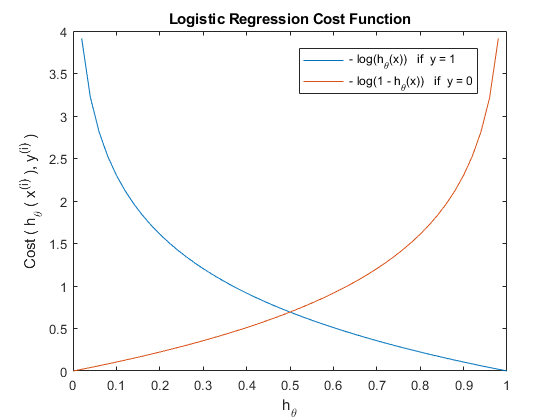
\includegraphics[scale=0.7]{W3_costlogistic}
\caption{Logistic Regression Cost Function}
\label{fig:W3_cost}
\end{figure}

The more our hypothesis is off from y, the larger the cost function output. If our hypothesis is equal to y, then our cost is 0:
\begin{align*}
& \mathrm{Cost}(h_\theta(x),y) = 0 \text{  if  } h_\theta(x) = y \\ 
& \mathrm{Cost}(h_\theta(x),y) \rightarrow \infty \text{  if  } y = 0 \; \mathrm{and} \; h_\theta(x) \rightarrow 1 \\ 
& \mathrm{Cost}(h_\theta(x),y) \rightarrow \infty \text{  if  } y = 1 \; \mathrm{and} \; h_\theta(x) \rightarrow 0 \\ 
\end{align*}
If our correct answer `y' is 0, then the cost function will be 0 if our hypothesis function also outputs 0. If our hypothesis approaches 1, then the cost function will approach infinity.

If our correct answer `y' is 1, then the cost function will be 0 if our hypothesis function outputs 1. If our hypothesis approaches 0, then the cost function will approach infinity.

Note that writing the cost function in this way guarantees that $J(\theta)$ is convex for logistic regression.

\section{Simplified Cost Function and Gradient Descent}
We can compress our cost function's two conditional cases into one case:

\begin{equation}
\mathrm{Cost}(h_\theta(x),y) = - y \; \log(h_\theta(x)) - (1 - y) \log(1 - h_\theta(x))
\end{equation}

Notice that when y is equal to 1, then the second term $(1-y)\log(1-h_\theta(x))$ will be zero and will not affect the result. If y is equal to 0, then the first term $-y \log(h_\theta(x))$ will be zero and will not affect the result.

We can fully write out our entire cost function as follows:

\begin{equation}
J(\theta) = - \frac{1}{m} \displaystyle \sum_{i=1}^m [y^{(i)}\log (h_\theta (x^{(i)})) + (1 - y^{(i)})\log (1 - h_\theta(x^{(i)}))]
\end{equation}

A vectorized implementation is:
\begin{align}
h &= g(X\theta)\\
J(\theta)  &= \frac{1}{m} \cdot \left(-y^{T}\log(h)-(1-y)^{T}\log(1-h)\right)
\end{align}

\subsection{Gradient Descent}
Remember that the general form of gradient descent is:
\begin{align*}
& Repeat \; \lbrace \\ 
& \; \theta_j := \theta_j - \alpha \dfrac{\partial}{\partial \theta_j}J(\theta) \\ 
& \rbrace
\end{align*}

We can work out the derivative part using calculus to get:

\begin{align*}
& Repeat \; \lbrace \\
& \; \theta_j := \theta_j - \frac{\alpha}{m} \sum_{i=1}^m (h_\theta(x^{(i)}) - y^{(i)}) x_j^{(i)} \\ & \rbrace
\end{align*}

Notice that this algorithm is identical to the one we used in linear regression. We still have to simultaneously update all values in theta.

A vectorized implementation is:
\[\theta := \theta - \frac{\alpha}{m} X^{T} (g(X \theta ) - \vec{y}) \]

\subsection{Partial derivative of Cost Function}

First calculate derivative of sigmoid function (it will be useful while finding partial derivative of $J(\theta)$

{\small
\begin{align*}
\sigma(x)'
&=\left(\frac{1}{1+e^{-x}}\right)'=\frac{-(1+e^{-x})'}{(1+e^{-x})^2}\\
&=\frac{-1'-(e^{-x})'}{(1+e^{-x})^2}=\frac{0-(-x)'(e^{-x})}{(1+e^{-x})^2}\\
&=\frac{-(-1)(e^{-x})}{(1+e^{-x})^2}=\frac{e^{-x}}{(1+e^{-x})^2} \\ 
&=\left(\frac{1}{1+e^{-x}}\right)\left(\frac{e^{-x}}{1+e^{-x}}\right)\\
&=\sigma(x)\left(\frac{+1-1 + e^{-x}}{1+e^{-x}}\right)\\
&=\sigma(x)\left(\frac{1 + e^{-x}}{1+e^{-x}} - \frac{1}{1+e^{-x}}\right)\\
&=\sigma(x)(1 - \sigma(x))
\end{align*}
}

Now we are ready to find out resulting partial derivative:
{\small
\begin{align*}
&\frac{\partial}{\partial \theta_j} J(\theta)= \\ 
&= \frac{\partial}{\partial \theta_j} \frac{-1}{m}\sum_{i=1}^m \left [ y^{(i)} log (h_\theta(x^{(i)})) + (1-y^{(i)}) log (1 - h_\theta(x^{(i)})) \right ] \\
&= - \frac{1}{m}\sum_{i=1}^m \left [     y^{(i)} \frac{\partial}{\partial \theta_j} log (h_\theta(x^{(i)}))   + (1-y^{(i)}) \frac{\partial}{\partial \theta_j} log (1 - h_\theta(x^{(i)}))\right ] \\
&= - \frac{1}{m}\sum_{i=1}^m \left [     \frac{y^{(i)} \frac{\partial}{\partial \theta_j} h_\theta(x^{(i)})}{h_\theta(x^{(i)})}   + \frac{(1-y^{(i)})\frac{\partial}{\partial \theta_j} (1 - h_\theta(x^{(i)}))}{1 - h_\theta(x^{(i)})}\right ] \\
&= - \frac{1}{m}\sum_{i=1}^m \left [     \frac{y^{(i)} \frac{\partial}{\partial \theta_j} \sigma(\theta^T x^{(i)})}{h_\theta(x^{(i)})}   + \frac{(1-y^{(i)})\frac{\partial}{\partial \theta_j} (1 - \sigma(\theta^T x^{(i)}))}{1 - h_\theta(x^{(i)})}\right ] \\
&= - \frac{1}{m}\sum_{i=1}^m \left [     \frac{y^{(i)} \sigma(\theta^T x^{(i)}) (1 - \sigma(\theta^T x^{(i)})) \frac{\partial}{\partial \theta_j} \theta^T x^{(i)}}{h_\theta(x^{(i)})}   + \frac{- (1-y^{(i)}) \sigma(\theta^T x^{(i)}) (1 - \sigma(\theta^T x^{(i)})) \frac{\partial}{\partial \theta_j} \theta^T x^{(i)}}{1 - h_\theta(x^{(i)})}\right ] \\
&= - \frac{1}{m}\sum_{i=1}^m \left [     \frac{y^{(i)} h_\theta(x^{(i)}) (1 - h_\theta(x^{(i)})) \frac{\partial}{\partial \theta_j} \theta^T x^{(i)}}{h_\theta(x^{(i)})}   - \frac{(1-y^{(i)}) h_\theta(x^{(i)}) (1 - h_\theta(x^{(i)})) \frac{\partial}{\partial \theta_j} \theta^T x^{(i)}}{1 - h_\theta(x^{(i)})}\right ] \\
&= - \frac{1}{m}\sum_{i=1}^m \left [     y^{(i)} (1 - h_\theta(x^{(i)})) x^{(i)}_j - (1-y^{(i)}) h_\theta(x^{(i)}) x^{(i)}_j\right ] \\
&= - \frac{1}{m}\sum_{i=1}^m \left [     y^{(i)} (1 - h_\theta(x^{(i)})) - (1-y^{(i)}) h_\theta(x^{(i)}) \right ] x^{(i)}_j \\
&= - \frac{1}{m}\sum_{i=1}^m \left [     y^{(i)} - y^{(i)} h_\theta(x^{(i)}) - h_\theta(x^{(i)}) + y^{(i)} h_\theta(x^{(i)}) \right ] x^{(i)}_j \\
&= - \frac{1}{m}\sum_{i=1}^m \left [ y^{(i)} - h_\theta(x^{(i)}) \right ] x^{(i)}_j  \\
&= \frac{1}{m}\sum_{i=1}^m \left [ h_\theta(x^{(i)}) - y^{(i)} \right ] x^{(i)}_j
\end{align*}
}

The vectorized version:
\begin{equation}
\nabla J(\theta) = \frac{1}{m} \cdot X^T \cdot \left(g\left(X\cdot\theta\right) - \vec{y}\right)
\end{equation}

\section{Advances Optimization}
\textbf{``Conjugate gradient"}, \textbf{``BFGS"}, and \textbf{``L-BFGS"} are more sophisticated, faster ways to optimize $\theta$ that can be used instead of gradient descent. A. Ng suggests not to write these more sophisticated algorithms yourself (unless you are an expert in numerical computing) but use the libraries instead, as they're already tested and highly optimized. Octave provides them.

We first need to provide a function that evaluates the following two functions for a given input value $\theta$:

\begin{align*}
J(\theta)\\
\frac{\partial}{\partial\theta_j}J(\theta)
\end{align*}

We can write a single function that returns both of these:

\begin{verbatim}
function [jVal, gradient] = costFunc(theta)
  jVal = [...code to compute J(theta)...];
  gradient = [...code to compute derivative of J(theta)...];
end
\end{verbatim}

Then we can use octave's \verb| fminunc()| optimization algorithm along with the \verb|optimset()| function that creates an object containing the options we want to send to \verb| fminunc()|. (Note: the value for MaxIter should be an integer, not a character string - errata in the video at 7:30)

\begin{verbatim}
options = optimset('GradObj', 'on', 'MaxIter', 100);
initTheta = zeros(2,1);
[optTheta, funcVal, exitFlag] = fminunc(@costFunc, initTheta, options);
\end{verbatim}

We give to the function \verb| fminunc()| our cost function, our initial vector of theta values, and the \textbf{options} object that we created beforehand.

\section{Multiclass Classification: One-vs-all}
Now we will approach the classification of data into more than two categories. Instead of $y = {0,1}$ we will expand our definition so that $y = {0,1...n}$.

In this case we divide our problem into n+1 (+1 because the index starts at 0) binary classification problems; in each one, we predict the probability that `y' is a member of one of our classes.

\begin{align*}
& y \in \lbrace0, 1 ... n\rbrace \\
& h_\theta^{(0)}(x) = P(y = 0 | x ; \theta) \\
& h_\theta^{(1)}(x) = P(y = 1 | x ; \theta) \\
& \cdots \\
& h_\theta^{(n)}(x) = P(y = n | x ; \theta) \\
& \mathrm{prediction} = \max_i( h_\theta ^{(i)}(x) )\\
\end{align*}

We are basically choosing one class and then lumping all the others into a single second class. We do this repeatedly, applying binary logistic regression to each case, and then use the hypothesis that returned the highest value as our prediction.

\section{ML: Regularization}
{\bf The Problem of Overfitting}
Regularization is designed to address the problem of overfitting.

High bias or underfitting is when the form of our hypothesis function h maps poorly to the trend of the data. It is usually caused by a function that is too simple or uses too few features. eg. if we take $h_\theta(x) = \theta_0 + \theta_1x_1 + \theta_2x_2$ then we are making an initial assumption that a linear model will fit the training data well and will be able to generalize but that may not be the case.

At the other extreme, overfitting or high variance is caused by a hypothesis function that fits the available data but does not generalize well to predict new data. It is usually caused by a complicated function that creates a lot of unnecessary curves and angles unrelated to the data.

This terminology is applied to both linear and logistic regression. There are two main options to address the issue of overfitting:

\begin{itemize}
  \item[1)] Reduce the number of features
  \begin{itemize}
  	\item[A)] Manually select which features to keep. 
  	\item[B)] Use a model selection algorithm (studied later in the course).
  \end{itemize}
  \item[2)] Regularization
  \begin{itemize}
  	\item[A)] Keep all the features, but reduce the parameters $\theta_j$
  	\item[B)] Regularization works well when we have a lot of slightly useful features.
  \end{itemize}  
\end{itemize}

\section{Cost Function}
f we have overfitting from our hypothesis function, we can reduce the weight that some of the terms in our function carry by increasing their cost.

Say we wanted to make the following function more quadratic:

$$\theta_0 + \theta_1x + \theta_2x^2 + \theta_3x^3 + \theta_4x^4$$

We'll want to eliminate the influence of $\theta_3x^3$ and $\theta_4x^4$. Without actually getting rid of these features or changing the form of our hypothesis, we can instead modify our \textbf{cost function}:
\begin{equation}
min_\theta\ \dfrac{1}{2m}\sum_{i=1}^m (h_\theta(x^{(i)}) - y^{(i)})^2 + 1000\cdot\theta_3^2 + 1000\cdot\theta_4^2
\end{equation}

We've added two extra terms at the end to inflate the cost of $\theta_3$ and $\theta_4$. Now, in order for the cost function to get close to zero, we will have to reduce the values of $\theta_3$ and $\theta_4$ to near zero. This will in turn greatly reduce the values of $\theta_3x^3$ and $\theta_4x^4$ in our hypothesis function.

We could also regularize all of our theta parameters in a single summation:

\begin{equation}
min_\theta\ \dfrac{1}{2m}\ \left[ \sum_{i=1}^m (h_\theta(x^{(i)}) - y^{(i)})^2 + \lambda\ \sum_{j=1}^n \theta_j^2 \right]
\end{equation}

The $\lambda$, or lambda, is \textbf{the regularization parameter}. It determines how much the costs of our theta parameters are inflated. You can visualize the effect of regularization in this \href{https://www.desmos.com/calculator/1hexc8ntqp}{interactive plot}

Using the above cost function with the extra summation, we can smooth the output of our hypothesis function to reduce overfitting. If lambda is chosen to be too large, it may smooth out the function too much and cause underfitting.

\section{Regularized Linear Regression}
We can apply regularization to both linear regression and logistic regression. We will approach linear regression first.

\subsection{Gradient Descent}
We will modify our gradient descent function to separate out $\theta_0$ from the rest of the parameters because we do not want to penalize $\theta_0$.
\begin{align*}
& \text{Repeat}\ \lbrace \\
& \ \ \ \ \theta_0 := \theta_0 - \alpha\ \frac{1}{m}\ \sum_{i=1}^m (h_\theta(x^{(i)}) - y^{(i)})x_0^{(i)} \\
& \ \ \ \ \theta_j := \theta_j - \alpha\ \left[ \left( \frac{1}{m}\ \sum_{i=1}^m (h_\theta(x^{(i)}) - y^{(i)})x_j^{(i)} \right) + \frac{\lambda}{m}\theta_j \right] &\ \ \ \ \ \ \ \ \ \ j \in \lbrace 1,2...n\rbrace\newline
& \rbrace
\end{align*}

The term $\frac{\lambda}{m}\theta_j$ performs our regularization.
With some manipulation our update rule can also be represented as:

\begin{equation}
\theta_j := \theta_j(1 - \alpha\frac{\lambda}{m}) - \alpha\frac{1}{m}\sum_{i=1}^m(h_\theta(x^{(i)}) - y^{(i)})x_j^{(i)}
\end{equation}

The first term in the above equation, $1 - \alpha\frac{\lambda}{m}$ will always be less than 1. Intuitively you can see it as reducing the value of $\theta_j$ by some amount on every update.

Notice that the second term is now exactly the same as it was before.

\subsection{Normal Equation}
Now let's approach regularization using the alternate method of the non-iterative normal equation.

To add in regularization, the equation is the same as our original, except that we add another term inside the parentheses:

\begin{align*}
& \theta = \left( X^TX + \lambda \cdot L \right)^{-1} X^Ty \\
& \text{where}\ \ L = 
\begin{bmatrix} 
0 & & & & \\ 
& 1 & & & \\ 
& & 1 & & \\ 
& & & \ddots & \\
& & & & 1 \\
\end{bmatrix}
\end{align*}

L is a matrix with 0 at the top left and 1's down the diagonal, with 0's everywhere else. It should have dimension $(n+1)\times(n+1)$. Intuitively, this is the identity matrix (though we are not including $x_0$), multiplied with a single real number $\lambda$.

Recall that if $m \leq n$, then $X^TX$ is non-invertible. However, when we add the term $\lambda \cdot L$, then $X^TX + \lambda \cdot L$ becomes invertible.
 
\section{Regularized Logistic Regression}
We can regularize logistic regression in a similar way that we regularize linear regression. Let's start with the cost function.
\subsection{Cost Function} 
Recall that our cost function for logistic regression was:
\begin{equation}
J(\theta) = - \frac{1}{m} \sum_{i=1}^m \left[ y^{(i)}\ \log (h_\theta (x^{(i)})) + (1 - y^{(i)})\ \log (1 - h_\theta(x^{(i)})) \right]
\end{equation}

We can regularize this equation by adding a term to the end:

\begin{equation}
\begin{split}
&J(\theta) = \\
&- \frac{1}{m} \sum_{i=1}^m \left[ y^{(i)}\ \log (h_\theta (x^{(i)})) + (1 - y^{(i)})\ \log (1 - h_\theta(x^{(i)}))\right] + \frac{\lambda}{2m}\sum_{j=1}^n \theta_j^2
\end{split}
\end{equation}	

\textbf{Note Well}: The second sum, $\sum_{j=1}^n \theta_j^2$ means to explicitly exclude the bias term, $\theta_0$. I.e. the $\theta$ vector is indexed from $\theta$ to n (holding n+1 values, $\theta_0$ through $\theta_n$), and this sum explicitly skips $\theta_0$, by running from 1 to n, skipping 0.

\subsection{Gradient Descent}
Just like with linear regression, we will want to \textbf{separately} pdate $\theta_0$ and the rest of the parameters because we do not want to regularize $\theta_0$.

\begin{align*}
& \text{Repeat}\ \lbrace \\
& \ \ \ \ \theta_0 := \theta_0 - \alpha\ \frac{1}{m}\ \sum_{i=1}^m (h_\theta(x^{(i)}) - y^{(i)})x_0^{(i)} \\
& \ \ \ \ \theta_j := \theta_j - \alpha\ \left[ \left( \frac{1}{m}\ \sum_{i=1}^m (h_\theta(x^{(i)}) - y^{(i)})x_j^{(i)} \right) + \frac{\lambda}{m}\theta_j \right] &\ \ \ \ \ \ j \in \lbrace 1,2...n\rbrace\\
& \rbrace
\end{align*}

This is identical to the gradient descent function presented for linear regression.
\section{Initial Ones Feature Vector}
\subsection{Constant Feature}
As it turns out it is crucial to add a constant feature to your pool of features before starting any training of your machine. Normally that feature is just a set of ones for all your training examples.

Concretely, if $X$ is your feature matrix then $X_0$ is a vector with ones.

Below are some insights to explain the reason for this constant feature. The first part draws some analogies from electrical engineering concept, the second looks at understanding the ones vector by using a simple machine learning example.

\subsection{Electrical Engineering}
From electrical engineering, in particular signal processing, this can be explained as DC and AC.

The initial feature vector X without the constant term captures the dynamics of your model. That means those features particularly record changes in your output y - in other words changing some feature $X_i$ where $i\neq0$ will have a change on the output y. AC is normally made out of many components or harmonics; hence we also have many features (yet we have one DC term).

The constant feature represents the DC component. In control engineering this can also be the steady state.

Interestingly removing the DC term is easily done by differentiating your signal - or simply taking a difference between consecutive points of a discrete signal (it should be noted that at this point the analogy is implying time-based signals - so this will also make sense for machine learning application with a time basis - e.g. forecasting stock exchange trends).

Another interesting note: if you were to play and AC+DC signal as well as an AC only signal where both AC components are the same then they would sound exactly the same. That is because we only hear changes in signals and $\Delta(AC+DC) = \Delta(AC)$

\subsection{Housing price example}
Suppose you design a machine which predicts the price of a house based on some features. In this case what does the ones vector help with?

Let's assume a simple model which has features that are directly proportional to the expected price i.e. if feature Xi increases so the expected price y will also increase. So as an example we could have two features: namely the size of the house in $[m2]$, and the number of rooms.

When you train your machine you will start by pretending a ones vector $X_0$. You may then find after training that the weight for your initial feature of ones is some value $\theta_0$. As it turns, when applying your hypothesis function $h_{\theta}(X)$ in the case of the initial feature you will just be multiplying by a constant (most probably $\theta_0$ if you not applying any other functions such as sigmoids). This constant (let's say it's $\theta_0$ for argument's sake) is the DC term. It is a constant that doesn't change.

But what does it mean for this example? Well, let's suppose that someone knows that you have a working model for housing prices. It turns out that for this example, if they ask you how much money they can expect if they sell the house you can say that they need at least $\theta_0$ dollars (or rands) before you even use your learning machine. As with the above analogy, your constant $\theta_0$ is somewhat of a steady state where all your inputs are zeros. Concretely, this is the price of a house with no rooms which takes up no space.

However this explanation has some holes because if you have some features which decrease the price e.g. age, then the DC term may not be an absolute minimum of the price. This is because the age may make the price go even lower.

Theoretically if you were to train a machine without a ones vector $f_{AC}(X)$, it's output may not  match the output of a machine which had a ones vector $f_{DC}(X)$. However, $f_{AC}(X)$ may have exactly the same trend as $f_{DC}(X)$ i.e. if you were to plot both machine's output you would find that they may look exactly the same except that it seems one output has just been shifted (by a constant). With reference to the housing price problem: suppose you make predictions on two houses $house_A$ and $house_B$ using both machines. It turns out while the outputs from the two machines would different, the difference between houseA and houseB's predictions according to both machines could be exactly the same. Realistically, that means a machine trained without the ones vector $f_AC$ could actually be very useful if you have just one benchmark point. This is because you can find out the missing constant by simply taking a difference between the machine's prediction an actual price - then when making predictions you simply add that constant to what even output you get. That is: if $house_{benchmark}$ is your benchmark then the DC component is simply $price(house_{benchmark}) - f_{AC}(features(house_{benchmark}))$.

A more simple and crude way of putting it is that the DC component of your model represents the inherent bias of the model. The other features then cause tension in order to move away from that bias position.

Kholofelo Moyaba

\subsection{A simpler approach}

A "bias" feature is simply a way to move the "best fit" learned vector to better fit the data. For example, consider a learning problem with a single feature $X_1$. The formula without the $X_0$ feature is just $theta_1 \ast X_1 = y$. This is graphed as a line that always passes through the origin, with slope y/theta. The $x_0$ term allows the line to pass through a different point on the y axis. This will almost always give a better fit. Not all best fit lines go through the origin (0,0) right?

Joe Cotton